\documentclass{article}

\usepackage{../preamble}
\standalonetrue

\pagestyle{fancy}
\fancyhf{}
\rhead{Section \thesection}
\lhead{MATH 316 Lecture 13}
\rfoot{Page \thepage}


\title{MATH 316 Lecture 13}
\author{Ashtan Mistal}
\date{June 02, 2021}

\begin{document}

\ifstandalone
\maketitle
\fi

\graphicspath{{./Lecture13/}}

Last time, we solved wave equations using the method of separation of variables, and introduced D'Alembert's solution. 

We found that D'Alembert's solution is in the following format:

$$y(x,t) = \frac{1}{2} \left[ f(x-at) + f(x+at) \right] + \frac{1}{2a} \int_{x-at}^{x+at} g(s) ds$$

This solution solves the following IBVP:

$$y_{tt} = a^2 y_{xx}$$

With initial conditions

$$y(x,0) = f(x), y_t(x,0) = g(x)$$

\section{Why do we use d'Alembert's method?}

\begin{itemize}
    \item It's very graphical (And you might like it more than series solutions)
\end{itemize}

Recall: Characteristic lines for wave equation are $x-at = \xi$ and $x+at = \eta$ are important for constructing the solution.  The initial data, $f(x)$ and $g(x)$ is propagated along these lines at speed of $a$. 

\section{Region of influence}

Let's consider $g(x) = 0$, i.e. no initial velocity. Suppose $y(x,0) = f(x)$ where $f(x)$ is defined on some finite interval $[-k, k]$. For example:

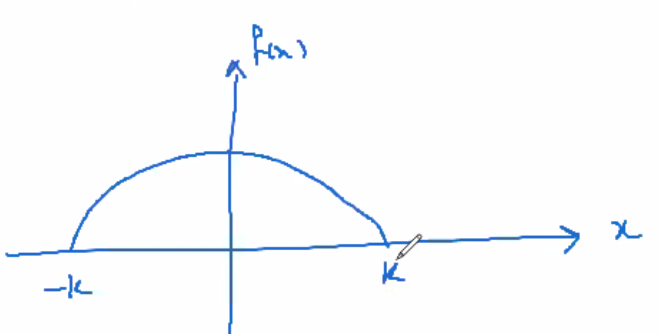
\includegraphics[width = 0.7 \textwidth]{image1.png}

$$y(t) = \frac{1}{2} \left[ f(x-at) + f(x+at) \right]$$

Sketch the characteristic curves. The domain is defined from $-k$ to $k$:

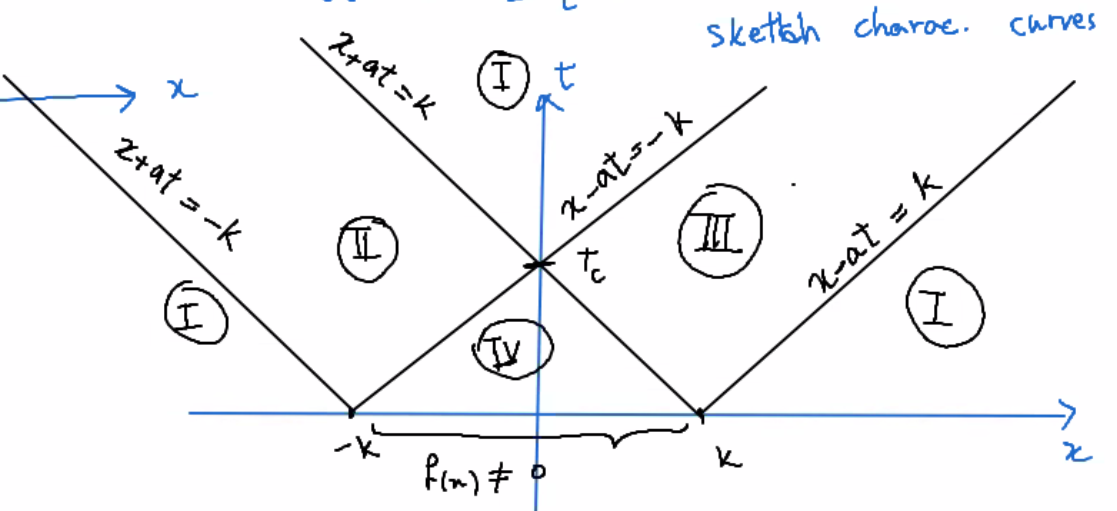
\includegraphics[width = 0.7 \textwidth]{image2.png}

Between $-k$ to $k$, $f(x) \neq 0$. 

$T_c$ is the critical time at which two waves become separate. 

\subsubsection{Regions}

\begin{itemize}
    \item Region 1:
    \begin{itemize}
        \item $y = 0$. (No initial displacement)
    \end{itemize}
    \item Region 2:
    \begin{itemize}
        \item $y(x,t) = \frac{1}{2} f(x+at)$. 
    \end{itemize}
    \item Region 3:
    \begin{itemize}
        \item $y(x,t) = \frac{1}{2} f(x-at)$
    \end{itemize}
    \item Region 4:
    \begin{itemize}
        \item Combination of both. We get characteristic lines from both 2 and 3:
        \item $y(x,t) = \frac{1}{2} \left[ f(x+at) + f(x-at) \right]$
    \end{itemize}
\end{itemize}

Regions 2, 3, and 4 are called regions of influence of $f(x)$ for $x \in [-k, k]$. 

\section{Domain of Dependence}

Suppose you know the solution $y(x_0, t_0)$ is the solution for $x \in [c,d]$. 

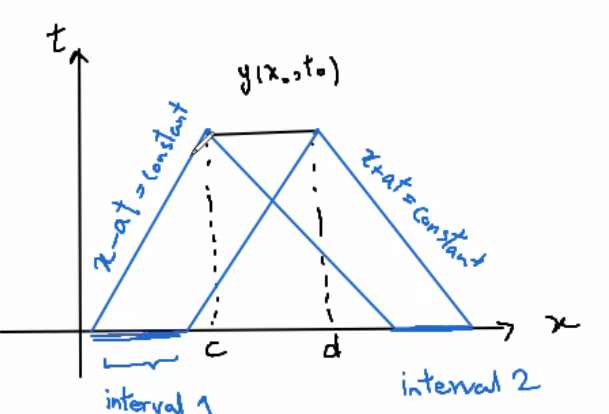
\includegraphics[width = 0.7 \textwidth]{image3.png}

Domain of dependence of the solution depends only on the initial data in interval 1, propagating right, and those data in interval 2 that are propagating left. 

\section{Examples}

\subsection{Example 10}

Assume we are given the wave equation:

$$y_{tt} = y_{xx}, -\infty < x < \infty$$

$$y(x,0) = \left\{ \begin{matrix} 1 & |x| < 1 \\ 0 & \text{otherwise} \end{matrix} \right.$$

$$y_t(x,0) = 0 = g(x)$$
\begin{center}
    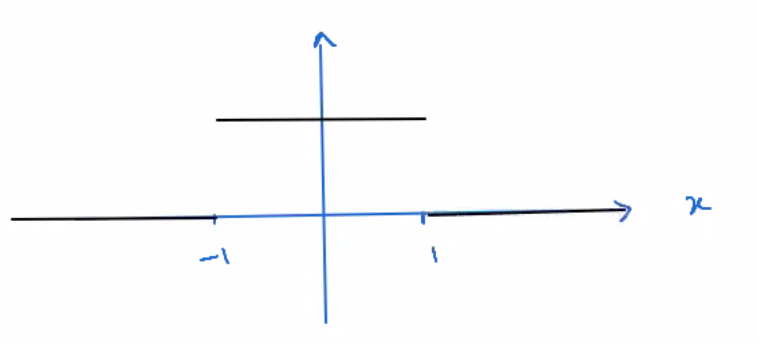
\includegraphics[width = 0.7 \textwidth]{image4.png}
\end{center}


From the D'Alembert formula, $y(x,t) = \frac{1}{2} \left[ f(x-t) + f(x+t) \right]$ given $a = 1$. 

\begin{center}
    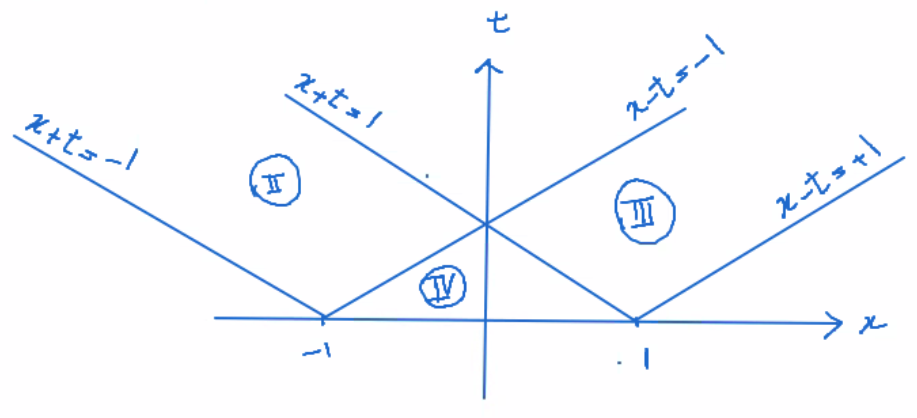
\includegraphics[width = 0.7 \textwidth]{image5.png}


At region 2, $y(x,t) = \frac{1}{2} f(x+t) = \frac{1}{2}$

\hfill

At region 3, $y(x,t) = \frac{1}{2} f(x-t) = \frac{1}{2}$

\hfill

At region 4, $y(x,t) = \frac{1}{2} \left[ f(x+t) + f(x-t) \right] = 1$

\end{center}

\subsection{Example 11}

$$y_{tt} = y_{xx}$$

$$y(0,t) = 0, y(1,t) = 0$$

Note: it has a boundary condition above. 

$$y(x,0) = \left\{ \begin{matrix} 0 & 0.00 \leq x < 0.45\\ 
10(x-0.45) & 0.45 \leq x < 0.50\\ 
20(0.55-x) & 0.50 \leq x < 0.55\\ 
0 & 0.55 \leq x \leq 1.00 \end{matrix} \right.$$

$$y_t(x,0) = 0 = g(x)$$

For Dirichlet we took the odd periodic extension and apply the D'Alembert solution. \footnote{Note that $F^o$ is the odd extension. }

$$y(x,t) = \frac{1}{2} \left( \underbrace{F^o (x-t)}_{\text{moving right}} + \underbrace{F^o (x+t)}_{\text{moving left}} \right)$$

The initial solution is given by:

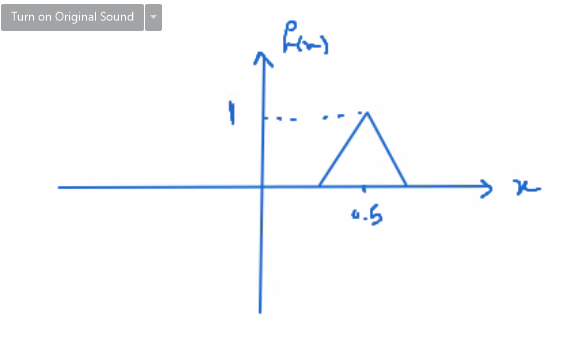
\includegraphics[width = 0.5 \textwidth]{image6.png}

Odd extension:

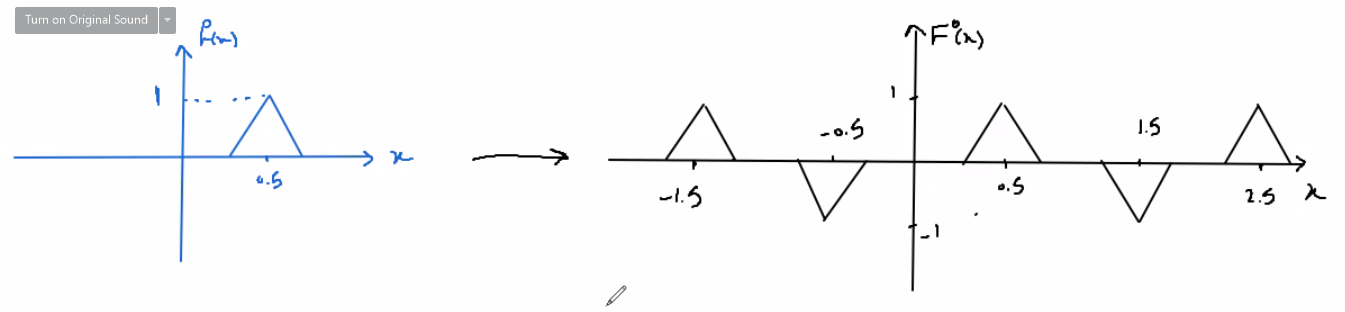
\includegraphics[width = 0.9 \textwidth]{image7.png}

Solution:

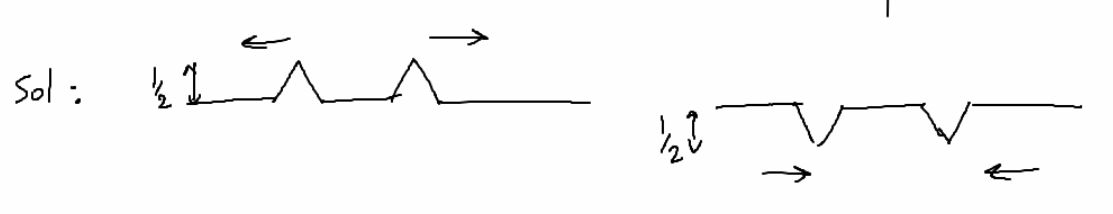
\includegraphics[width = 0.9 \textwidth]{image8.png}

Find $y(x,t) = y(0,1, 0.6)$:

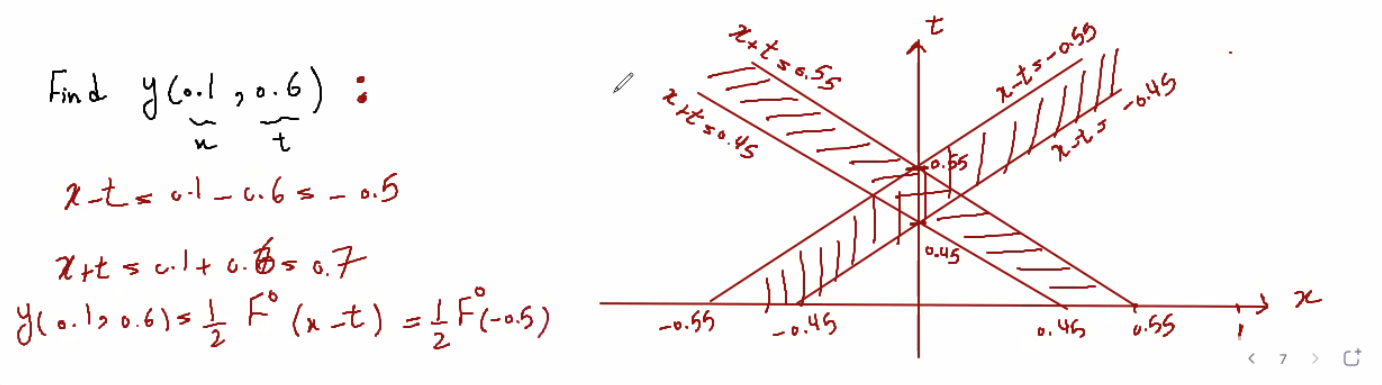
\includegraphics[width = 0.9 \textwidth]{image9.png}

Note that $\frac{1}{2} F^o (-0.5) = - \frac{1}{2} f(0.5) = - \frac{1}{2} (20 (0.55 - 0.5)) = -\frac{1}{2}$

\section{Laplace Equations PDF}

Firstly, for Laplace equations, we go through the 6 page pdf attached below.

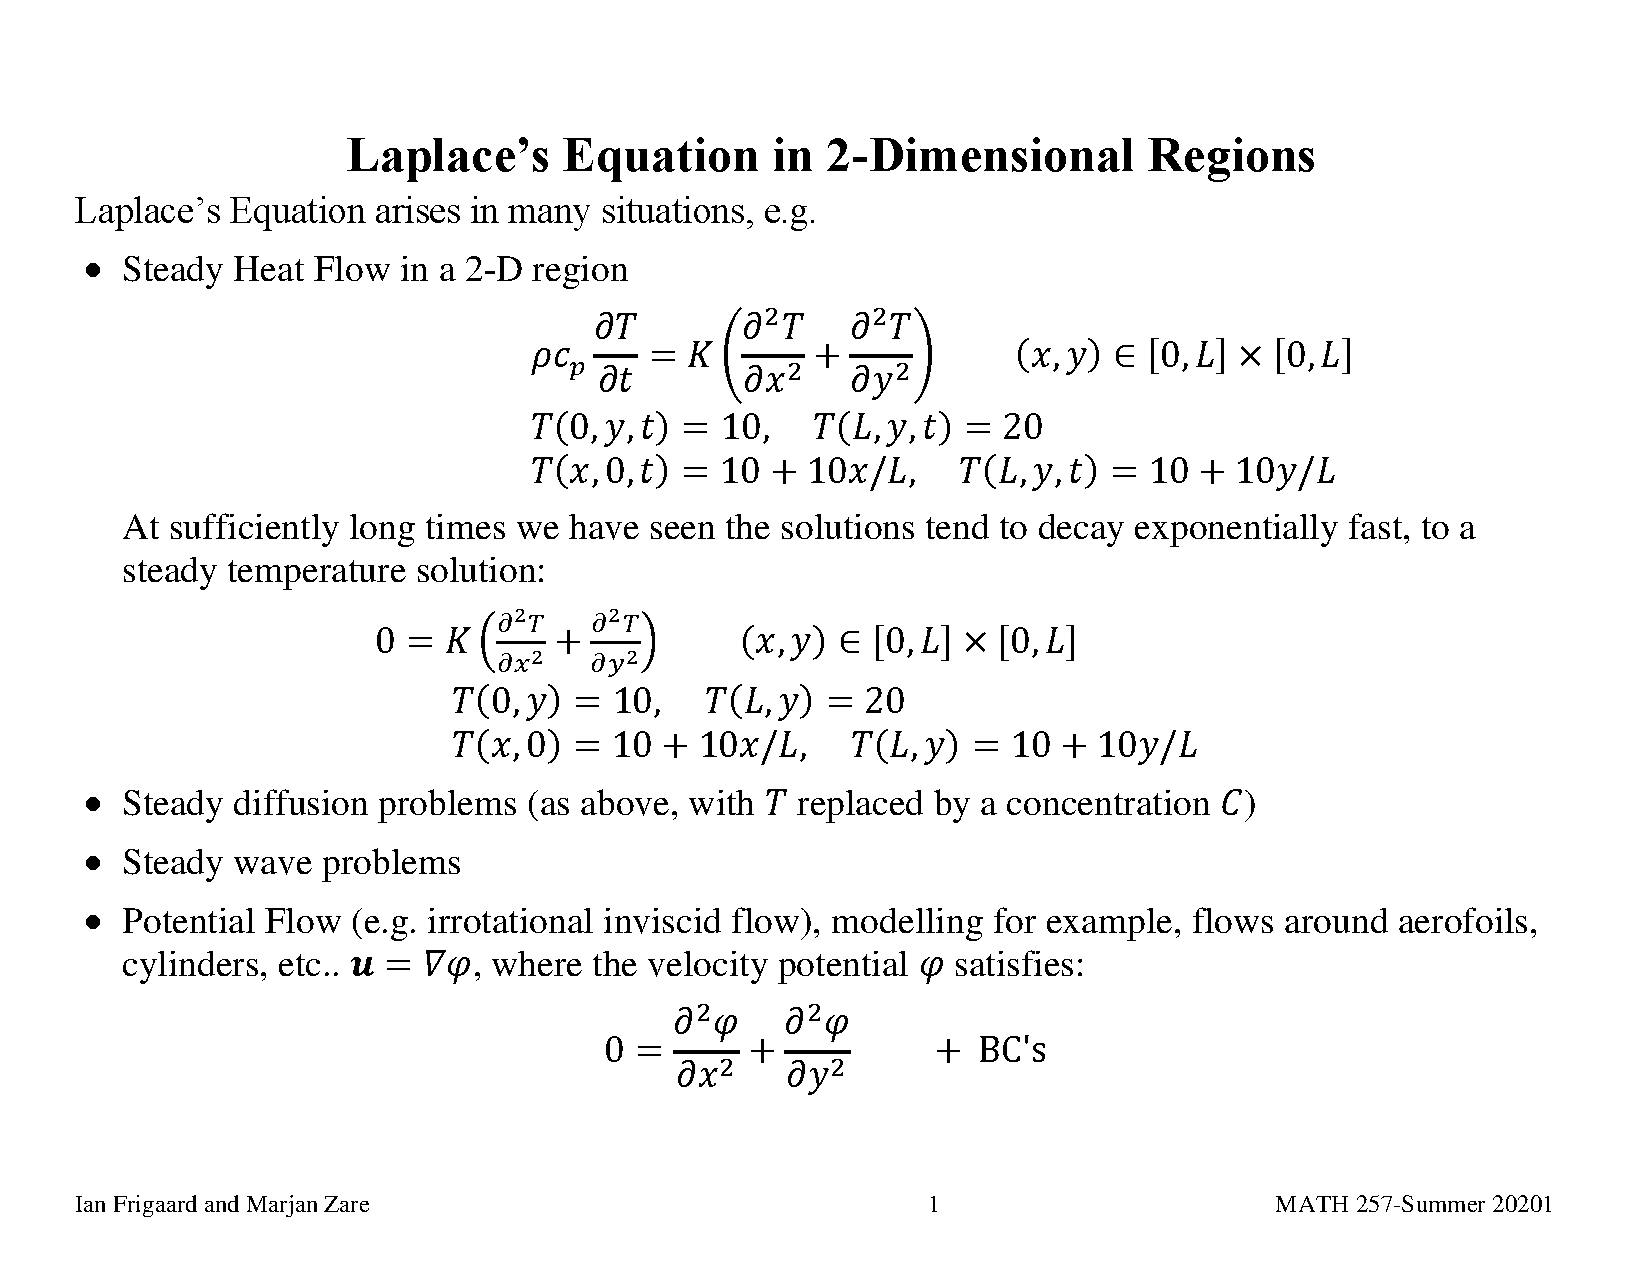
\includegraphics[page=1, width = 0.8 \textwidth]{Laplace Equation.pdf}

\includegraphics[page=2, width = 0.8 \textwidth]{Laplace Equation.pdf}

\includegraphics[page=4, width = 0.8 \textwidth]{Laplace Equation.pdf}

\includegraphics[page=5, width = 0.8 \textwidth]{Laplace Equation.pdf}

\includegraphics[page=6, width = 0.8 \textwidth]{Laplace Equation.pdf}

\section{Laplace Equations Notes}

$$\frac{\partial^2 u}{\partial x^2} + \frac{\partial^2 u}{\partial y^2} = 0 \to \Delta u = 0$$

where $\Delta$ is the laplacian. 

The main idea is to split into 4 problems, each with 3 homogeneous boundary conditions. 

[Using N,S,E,W notation]:

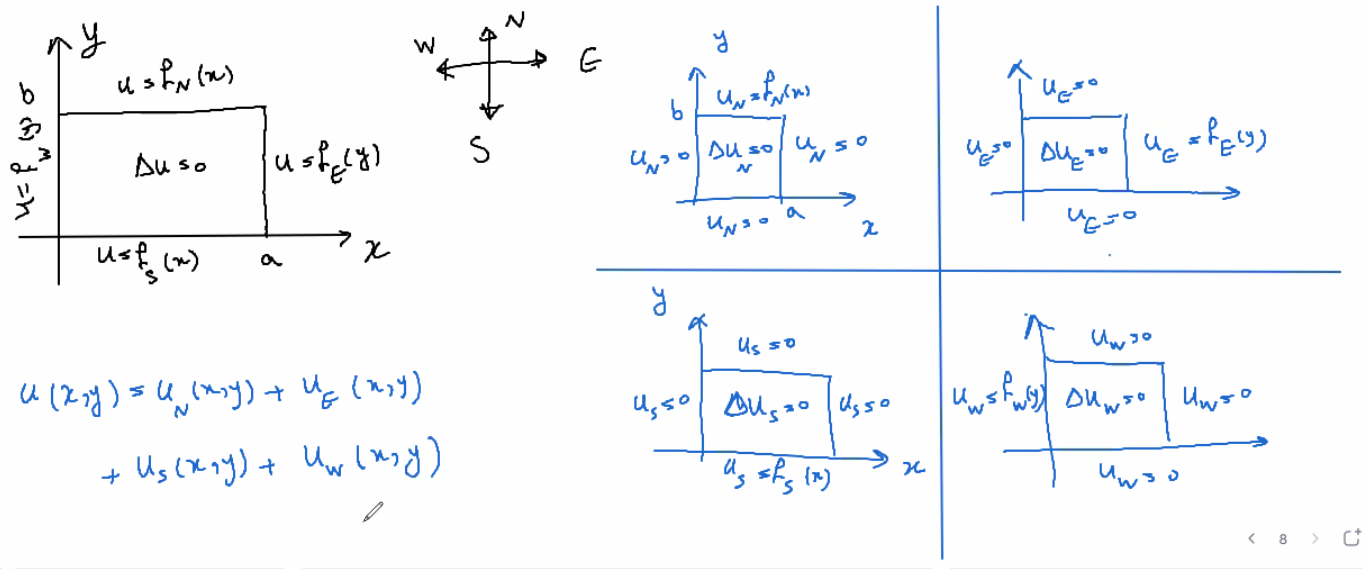
\includegraphics[width = 0.95 \textwidth]{image11.png}

\end{document}